\documentclass{article}
\usepackage[utf8]{inputenc}
\usepackage[T1]{fontenc}
\usepackage{graphicx}
\usepackage{algorithm}
\usepackage{algpseudocode}

\usepackage{listings}
\usepackage{xcolor}
\usepackage[margin=2cm]{geometry}
\usepackage{float}

\usepackage{amssymb} %Ajoute des symboles mathématiques comme R, Z, forall, exists, etc....
\usepackage{amsmath}
\usepackage{amsthm}


\lstdefinestyle{monstyle}{
    backgroundcolor=\color{white},
    commentstyle=\color{gray},
    keywordstyle=\color{blue},
    numberstyle=\tiny\color{gray},
    basicstyle=\ttfamily\small,
    breaklines=true,
    numbers=left,
    numbersep=5pt,
    frame=single,
}
\lstset{style=monstyle}


\title{\textbf{Rapport de TD n°4: Initiation à l'algorithmique}}
\author{Derrez Lorenzo}

\begin{document}
\maketitle

\section*{\textbf{Exercice 1}}

\subsection*{Question 1:}

On a l'équation,
\[
    \# (n) = 1 + 2 \# (\frac{n}{2}).
\]
\\[0.3em]
Donc, 
\begin{itemize}
    \item $ a = 2 $ appels récursifs.
    \item $ b = 2 $ la division de la taille de l'entrée.
    \item $ k = 0 $ l'exposant de $ \# division + \# recomposition $.
\end{itemize}
Par le cours, on obtient (cas où $a>b^k$), 
\[
    \theta(n^{\log_b(a)})
\]
Finalement la solution est ; $ \theta(n) $.
\\[0.3em]
Optimalité : La solution donnée est en $\theta$ donc elle est optimale.

\subsection*{Question 2:}


\begin{itemize}
    \item Une définition naïve récursive est, pour un tableau T de taille n;
    \subitem $ \textit{LongMaxPlateau}(n) = max(\textit{LongMaxPlateau}(n_{gauche}), \textit{LongMaxPlateau}(n_{droit})) $
    \item C'est un définition erronée car : 
    \subitem elle ne s'applique aps correctement pour une entrée contenant la longueur maximale du plateau au milieu de T, et non au début ou à la fin de T.
    \item Par exemple : $ T = [2, 1, 2, 2, 2, 2, 1, 2], n = 8. $
    \item La définition récurisve naïve va içi renvoyer le max entre les tableaux gauche et droit. Or ces deux appels vont valoir 2 et dans ce cas, l'output renvoyé sera différent de 4 qui est l'output attendu pour cet exemple.
\end{itemize}

\subsection*{Question 3:}

Entrée : \textit{T} un tableau d'entiers, et deux indices \textit{i, j} $\leq 2$ qui délimitent la zone $ T[i..j[.$
\\
Sortie : un triplet $ (m_g, m, m_d) $ où, 
    \begin{itemize}
        \item $m_g$ est la longueur du plateau collé au début de la zone (il commence en $i$ et finit en $ i + m_g - 1$).
        \item $m$ est la longueur maximale d'un plateau dans la zone 
        \item $m_d$ est la longueur du plateau collé à la fin de la zone (il commence en $ j - m_d$ et finit en $ j - 1 $).
    \end{itemize}
Le milieu est $ c = (i+j)//2$. On a deux appels, 
\begin{itemize}
    \item $ S = (m_g, m, m_d) $ pour la zone gauche $ [i, c[ $ de taille $c-i$.
    \item $ U = (m_g, m, m_d) $ pour la zone droite $ [c, j[ $ de taille $j-c$.
\end{itemize}
Cas par défaut (aucun plateau ne traverse le milieu), 
\begin{itemize}
    \item $m_g = m_{g_1}$
    \item $m = \max(m_1, m_2)$
    \item $ m_d = m_{d_2}$
\end{itemize}
Si T[c-1] = T[c] (un plateau traverse le milieu), on corrige : 
\begin{itemize}
    \item $ m = \max(m_1, m_2, m_{d_1} + m_{g_2})$ 
    \item si $ m_{g_1} = c-i $ (la gauche est entièrement un plateau), alors $m_g = m_{g_1} + m_{g_2}$
    \item si $ m_{d_2} = j-c $ (la droite est entièrement un plateau), alors $m_d = m_{d_1} + m_{d_2}$
\end{itemize}

\subsection*{Question 4:}
\begin{lstlisting}[language=Python, caption={lmpRec}]
def lmpRec( T : Array[integer], i : integer, j : integer)-> (integer, integer, integer): 
    if j-i < 2:
        return (j-i, j-i, j-i) #zone vide ou 1 element
    c = (i+j)//2
    S = lmpRec(T, i, c) # (mg1, m1, md1)
    U = lmpRec(T, c, j) # (mg2, m2, md2)
    mg, m, md = S[0], max(S[1], U[1]), U[2]
    if T[c-1] == T[c]:
        m = max(m, S[2] + U[0])
        if S[0] == c-i:
            mg = S[0] + U[0]
        if U[2] == j-c:
            md = U[2] + S[2]
    return (mg, m, md)
\end{lstlisting}

\subsection*{Question 5:}
Pour réaliser l'arbre d'appels en entier, on peut l'écrire de la manière suivante : 

\begin{minipage}[c]{15cm}
    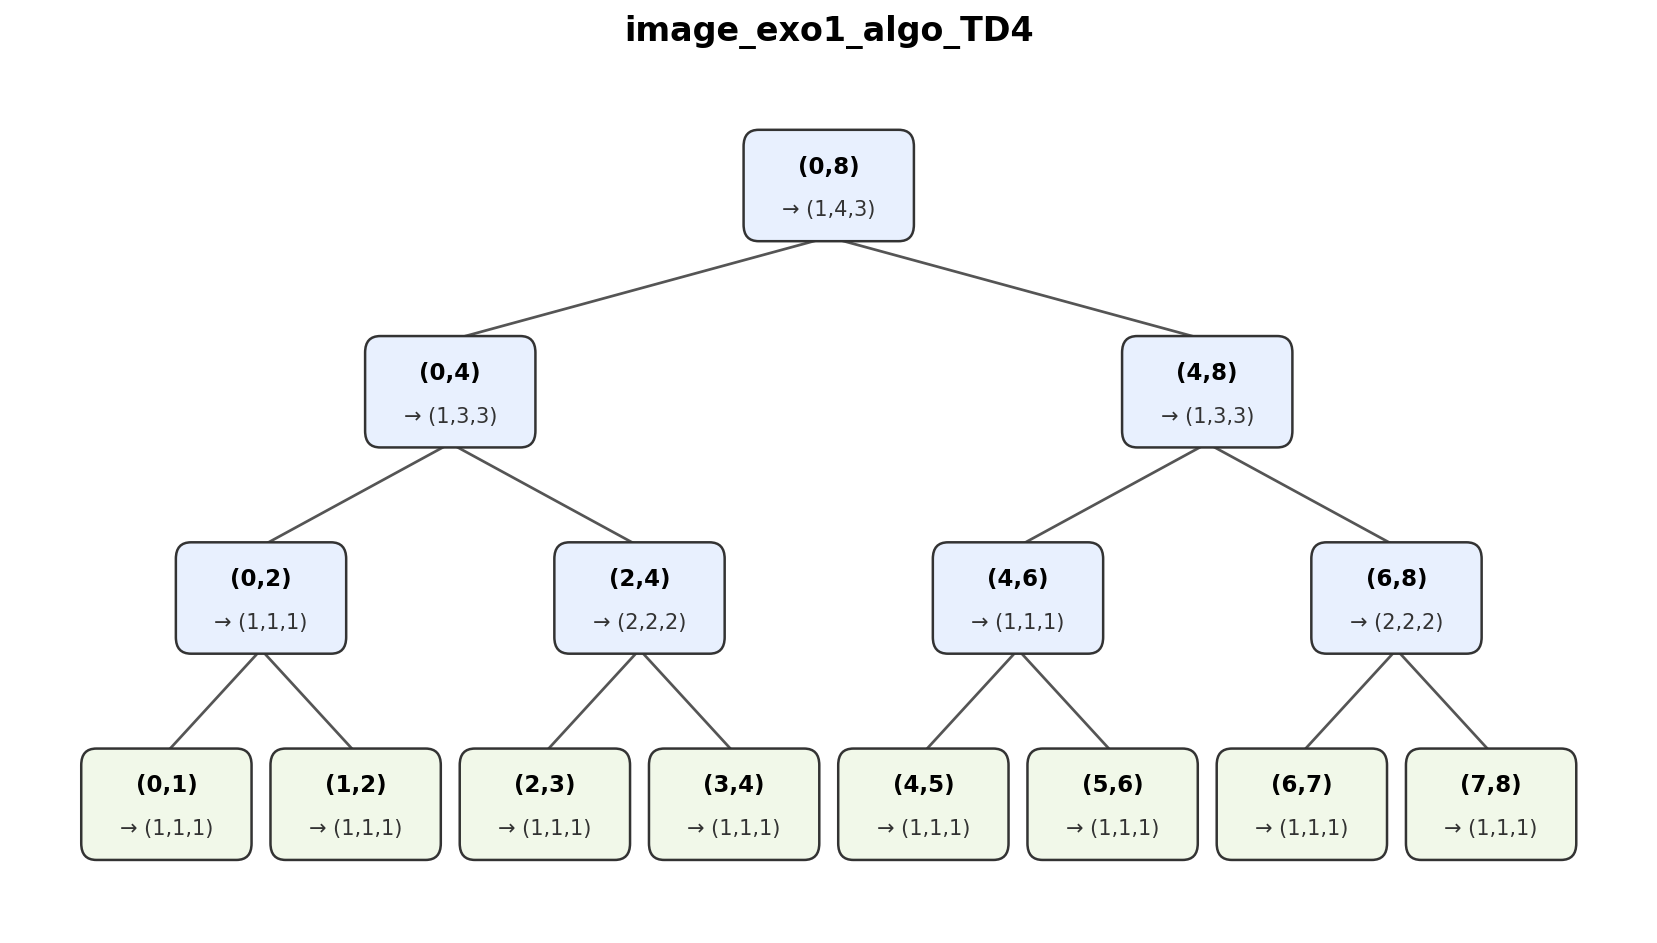
\includegraphics[width=15cm]{image_exo1_algo_TD4.png}
\end{minipage}

\subsection*{Question 6:}
Complexité en espace : 
\begin{itemize}
    \item Déterminer la capacité maximale utilsiée à un instant de l'exécution.
    \item Durant chaque appel, on stock : 
    \subitem S, U, i, j, mg, md $ \longrightarrow \theta(1) $
    \item S et U ne sont pas simultané : 
    \subitem on regarde le max de la mémoire, pas la somme.
    \item L'espace se définit pour n la taille de l'entrée : 
\end{itemize}
\[ E(n) = (\text{espace local}) + \max(E(\frac{n}{2}), E(\frac{n}{2})) \]
Entre autres, 
\[
    E(n) = 1 + E(\frac{n}{2})\times 1
\]  
où $ a = 1, b = 2, k = 0$.
\\
Par le cours, on obtient, 
\[
    \theta(\log(n)) \text{ en espace.}
\]
Par ailleurs, il y a $ 1 + \log_2(n) $ appels.

\section*{\textbf{Exercice 2}}

\subsection*{Question 1:}

\begin{figure}[H]
    \centering
    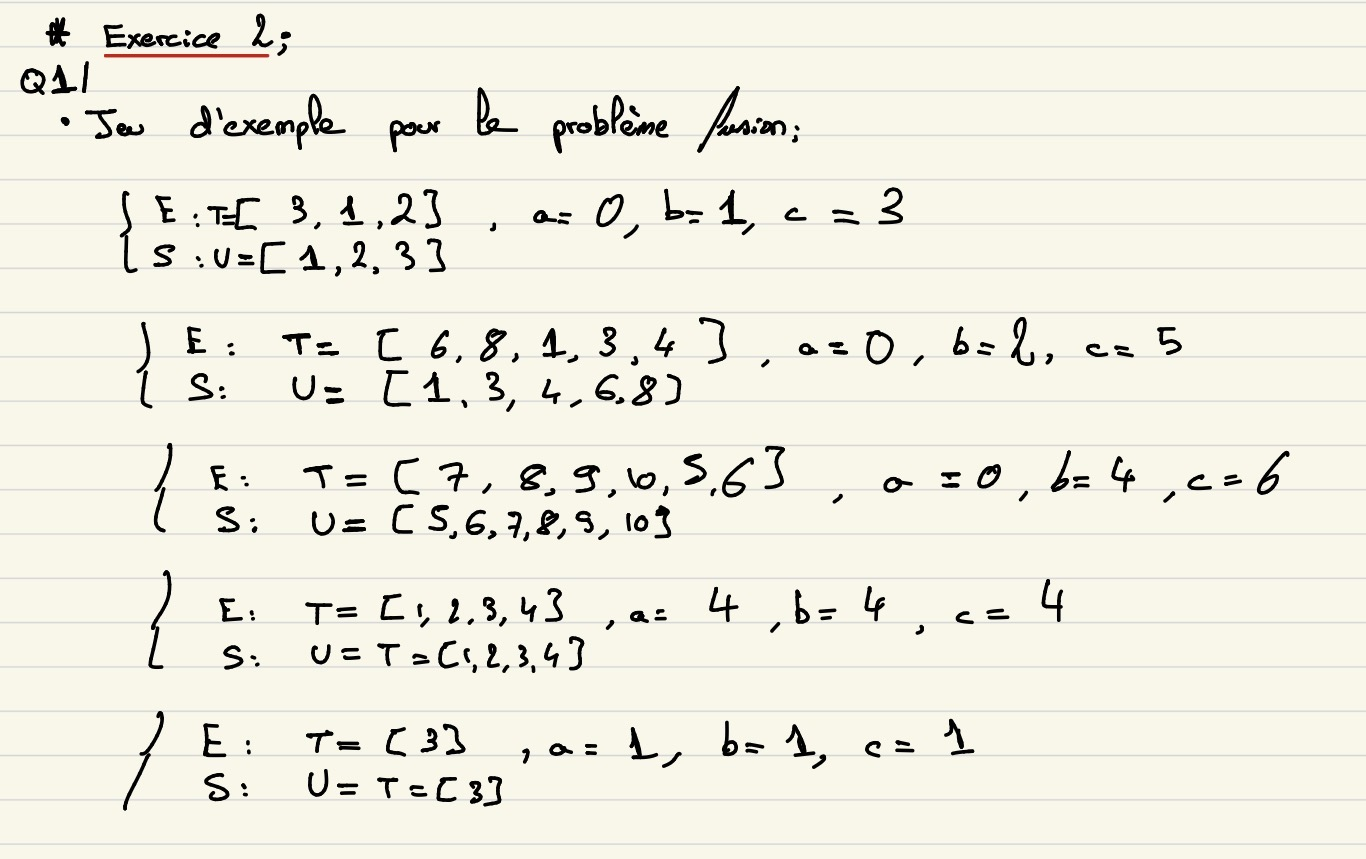
\includegraphics[width=\textwidth]{jeu_test_exo2_TD4.png}
    \caption{Jeu d'exemples pour le problème de FUSION.}
\end{figure}

\subsection*{Question 2}

\begin{algorithm}[H]
    \centering
    \caption{Solution Algorithmique de \textit{FUSION}}
    \begin{algorithmic}[1]
        \State Entrée : un tableau T d'entiers, a, b et c des entiers vérifiant : $ 0 \leq a \leq b \leq c \leq size(T) $
        \State Sortie : un tableau U d'entiers tel que 
        \begin{itemize}
            \item U[0:a] = T[0:a]
            \item U[c : |U|] = T[c : |T|]
            \item U[a : c] et T[a : c] ont memes valeurs (avec memes nombre d'occurrence) 
            \item Si T[a:b] et T[b:c] sont triés alors U[a:c] est trié.
        \end{itemize}
        \Function {FUSION}{(T : Array[integer], a:int, b:int, c:int) -> Array[integer]}:
            \State int n $\leftarrow$ size(T) 
            \State U $\leftarrow$ newArray(n, 0)
            \State int k $\leftarrow$ 0
            \State Tant que k < a : 
                \State \quad U[k] $\leftarrow$ T[k]
                \State  \quad k $\leftarrow$ k + 1
            \State int i $\leftarrow$ a 
            \State int j $\leftarrow$ b 

            \State Tant que i < b et j < c: 
                \State \quad Si T[i] $\leq$ T[j]:
                    \State \qquad U[k] $\leftarrow$ T[i]
                    \State \qquad i $\leftarrow$ i + 1
                \State \quad Sinon 
                    \State \qquad U[k] $\leftarrow$ T[j]
                    \State \qquad j $\leftarrow$ j + 1
                \State \quad k $\leftarrow$ k + 1
            \State Tant que i < b:
                \State \quad U[k] $ \leftarrow $ T[i]
                \State \quad k $ \leftarrow $ k + 1
                \State \quad i $ \leftarrow $ i + 1
            \State Tant que j < c: 
                \State \quad U[k] = T[j]
                \State \quad j $\leftarrow$ j + 1
                \State \quad k $\leftarrow$ k + 1
            \State Tant que k < n :
                \State \quad U[k] $\leftarrow$ T[k]
                \State \quad k $\leftarrow$ k + 1
            \State \Return U
        \EndFunction
    \end{algorithmic}
\end{algorithm}

La complexité est en $\theta(n)$ en temps et en espace, où $n$ est la taille de $T$.

\subsection*{Question 3:}

\begin{itemize}
    \item Actuellement, à chaque appel de la fonction \textit{FUSION}, on crée un nouveau tableau U.
    \item On pourrait creer une fonction \textit{TRI\_FUSION}dans laquelle on crée U une seule fois et on utilise \textit{FUSION} comme une fonction auxiliaire avec U en paramètre.
    \item Cette méthode réduit le nombre d'appels à la création de U. 
    \item Toutefois, la complexité en espace reste $\theta(n)$ car il s'agit de la mémore maximale utilisée lors de l'exécution et non le nombre total de créations, et la création de U est linéaire en n.
\end{itemize}

\end{document}